\section{Hybrid force position controller}
In this section the hybrid force position controller is presented.
With reference to the quantities introduced in the section \ref{sec:frames}
this controller should allow to regulate the position and the attitude of the hand
with respect to the frame $\{S_{ws}\}$ and at the same time the contact force between
the hand and the object expressed along the $z$ axis of the same frame.

\subsection{Desired dynamics of the error}\label{sec:desired_dyn}
In order to express the desired dynamics of the controlled system
more precisely the following error quantities are introduced
\[
e_x(t) =   \prescript{ws}{} r_{x,des}(t) - \prescript{ws}{} r_{x}(t)
\]
\[
e_y(t) =   \prescript{ws}{} r_{y,des}(t) - \prescript{ws}{} r_{y}(t)
\]
\[
\vec{e}_{\Phi}(t) = \vec{\Phi}_{des}(t) - \vec{\Phi}(t)
\]
where $\vec{r}$ is the vector from the origin $W$ of the frame $\{S_{ws}\}$ to the
center of the palm of the hand (see section \ref{sec:frames}) and $\vec{\Phi}$ is
a vector containing three angles that represent the orientation of the hand with respect
to the frame $\{S_{ws}\}$.
Also an error $e_z$ is defined as
\[
e_{z}(t) = \prescript{ws}{} F_{z,des}(t) - \prescript{ws}{} F_{z}(t)
\]
where $\prescript{ws}{} F_{z}$ is the force exerted by the hand on the object expressed
along the $\hat{\vec{k}}_{ws}$ direction.
\par
Using these definitions the desired dynamics of the error is expressed as
\[
\ddot{e}_{x} + B_x \dot{e}_x + K_x e_x = \vec{0} %\prescript{ws}{}{F}_x\\
\]
\[
\ddot{e}_{y} + B_y \dot{e}_y + K_y e_y = \vec{0} %\prescript{ws}{}{F}_y\\
\]
\[
\ddot{\vec{e}}_{\Phi} + B_{\Phi} \dot{\vec{e}}_{\Phi} + K_{\Phi} \vec{e}_{\Phi} = \vec{0} %\prescript{ws}{}{M}
\]
\[
e_z \xrightarrow[t \to \infty]{} 0
\]
The first two equations express the fact that the end-effector should rigidly follow
a given trajectory on a plane parallel to the surface of the table in a second order damped
fashion ($K$ and $B$ represent the proportional and damping terms).
The same reasoning applies for the attitude (third equation).
Finally the fourth equation only requires that the steady state force error should be zero.

\subsection{Definition of a state vector}
In order to develop a controller with the features described above
an \emph{operational} state space vector is defined as
\begin{equation}
  \label{eq:state_space}
  \prescript{ws}{}{\vec{x}} = 
  \begin{bmatrix}
    \prescript{ws}{} r_x & \prescript{ws}{} r_y & \prescript{ws}{}r_z & \psi & \theta & \phi
  \end{bmatrix}^T
\end{equation}
where the angles $\psi$, $\theta$ and $\phi$ are the Euler ZYZ parametrization of the rotation matrix
$\prescript{ws}{}{R}_{ee}$ between the frames $\{S_{ws}\}$ and $\{S_{ee}\}$
\[
\prescript{ws}{}{R}_{ee} = R_{ZYZ}(\psi, \theta, \phi) = R_{ZYZ}(\vec{\Phi})
\]
Even though the force $\prescript{ws}{} F_z$ does not appear directly in the state vector
by making the hypothesis that the second derivative of the state can be commanded arbitrarily
\begin{equation}\label{eq:ddx_acmd}
\prescript{ws}{}{\ddot{\vec{x}}} = \vec{a}_{cmd}
\end{equation}
it will be shown that force can be regulated by an appropriate choice of term $\vec{a}_{cmd}$.
The hypothesis made above is a strong one and will be relaxed in the section \ref{sec:invdyn}
where an inverse dynamics inner loop controller will be developed for the manipulator.
This kind of controller allows to transform the non-linear dynamics of the manipulator in a
double integrator system of the form (\ref{eq:ddx_acmd}).

\subsection{Hybrid Impedance control strategy}
Among the various works on force control strategies available in the robot control
literature the strategy called \emph{Hybrid Impedance Control} proposed by Anderson and Spong
\cite{Anderson1988} was chosen due to its generality.
\par
The Hybrid impedance controller (HIC) combines the hybrid force/position control
with an impedance based control approach.
\par
Hybrid force/position control was first proposed by Raibert and Craig \cite{Raibert1981} and
allows to assign different control strategies to each 
Cartesian degree of freedom using some selection matrices. However it neglects the
importance of the manipulator impedance as seen by the environment during the interaction with it.
\par
The concept of impedance proposed by Anderson an Spong is more general with respect to the common
impedance approach in which a PD position controller is implemented with position and velocity
feedback gains adjusted to obtain different apparent impedances. First of all the
impedance control is performed in operational space so that an apparent impedance can be imposed
regardless of the configuration of the manipulator. Moreover the concept of impedance proposed
allows to synthesize \emph{direct force} control schemes by matching a given ``environment impedance''
with the appropriate ``manipulator impedance''.
\par
In the following the HIC approach is explained in more details
and a control law $\vec{a}_{cmd}$ is designed in order to fulfill
the control objectives described in \ref{sec:desired_dyn}.

\subsection{Frequency domain impedances}
A central concept in the HIC framework is that of frequency domain impedances.
A complex number of the form 
\begin{equation}
  \label{eq:impedance}
  Z(\omega)=R(\omega)+jX(\omega)
\end{equation}
with real part $R(\omega)$ and imaginary part $X(\omega)$, which resembles the Laplace
transform between a generalized effort and flow for a linear system, is used to model
both the environment and the manipulator \emph{for each} degree of freedom
avilable. It should be noted that in this framework
the environment is defined to be any element connected to or
contacting the robot anywhere past the wrist force sensor.
\begin{figure}[h]
  \centering
  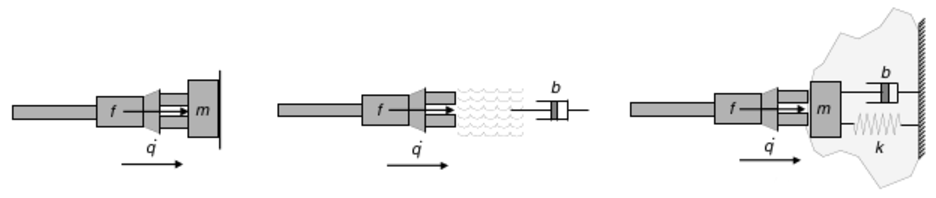
\includegraphics[scale=0.9]{type_of_impedances.pdf}
  \caption{Type of impedances. \label{fig:type_of_impedances}}
\end{figure}
\par
Impedances can be classified depending upon their \emph{low-frequency} behavior.
As $\omega$ approaches zero, one of three things can happen to 
the magnitude of the environment's and robot's impedance. It can 
approach infinity, it can approach a non-zero finite number or it can approach zero.
The following classification is now introduced:
\begin{itemize}
\item A system with impedance given by  (\ref{eq:impedance}) is \emph{inertial} IFF $\lim_{\omega \to 0}|Z(\omega)| = 0$ (Fig. \ref{fig:type_of_impedances}.a)
\item A system with impedance given by  (\ref{eq:impedance}) is \emph{resistive} IFF $\lim_{\omega \to 0}|Z(\omega)| = c$ where $0<c<\infty$ (Fig. \ref{fig:type_of_impedances}.b)
\item A system with impedance given by  (\ref{eq:impedance}) is \emph{capacitive} IFF $\lim_{\omega \to 0}|Z(\omega)| = \infty$ (Fig. \ref{fig:type_of_impedances}.c)
\end{itemize}

Capacitive, inertial and resistive systems are usually described in terms of 
Norton and Thèvenin equivalents. A capacitive system is 
represented by an impedance in parallel with a flow source (Norton).
An inertial system is represented by impedance in series with an 
effort source (Thévenin). Finally a resistive system 
can be either represented by a Thèvenin or Norton equivalent.

\subsection{The duality principle}
Once the environment has been properly modelled, the 
desired manipulator response may be determined. A fundamental goal for 
designing a controller is zero steady-state error to a step 
input. This will be obtained if the following duality principle is applied.
\begin{dualityprinciple}
  The manipulator should be controlled to respond as the dual of the environment.
\end{dualityprinciple}
This principle is most easily described in terms of Norton and Thèvenin equivalents.
An inertial environment, represented using a Thèvenin equivalent (Fig. \ref{fig:position_control_model}), is controlled by a manipulator represented by a non-inertial impedance.
\begin{figure}[h]
  \centering
  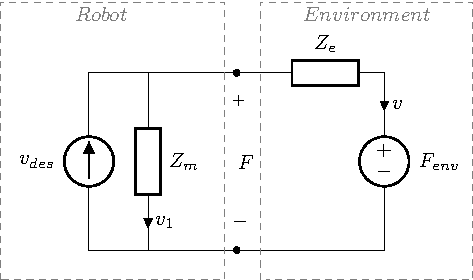
\includegraphics[scale=0.9]{position_control_model.pdf}
  \caption{Inertial environment. \label{fig:position_control_model}}
\end{figure}
Using the superposition principle the current (velocity) $v$ can be evaluated
\begin{equation}
  \label{eq:position_control_circuit}
  v = \frac{Z_m(s)}{Z_m(s) + Z_e(s)}v_{des} - 		\frac{F_{env}}{Z_e + Z_m}
\end{equation}
and the steady state error, assuming no environmental input ($F_{env} \equiv 0$) is equal to 
\[
e_{ss} \Big|_{F_{env}(t) \equiv 0} = \lim_{s \to 0}(v - v_{des}) = \frac{-Z_e(0)}{Z_m(0) + Z_e(0)}
\]
Since the the environment is inertial by hypothesis ($|Z_e(0)| = 0$) a choice of a non-inertial manipulator impedance ($Z_m(0) \neq 0$)
assures that
\[
e_{ss} \Big|_{F_{env}(t) \equiv 0} = 0
\]
So inertial environments are position controlled with a non-inertial manipulator impedances.
\par
A capacitive environment, represented using a Norton equivalent (Fig. \ref{fig:force_control_model}), 
is controlled by a manipulator represented by a 
non-capacitive impedance.
\begin{figure}[h]
  \centering
  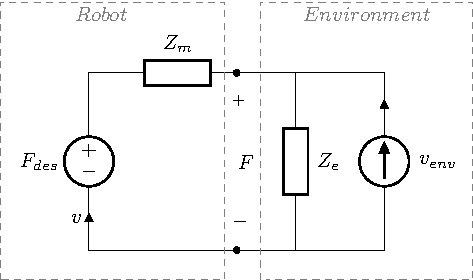
\includegraphics[scale=0.9]{force_control_model.pdf}
  \caption{Capacitive environment. \label{fig:force_control_model}}
\end{figure}
Using the superposition principle the voltage (force or torque) $F$ can be evaluated
\begin{equation}
  \label{eq:force_control_circuit}
  F = \frac{Z_e(s)}{Z_m(s) + Z_e(s)}F_{des} + \frac{Z_e Z_m}{Z_m + Z_e} V_{env}
\end{equation}

and the steady state error, assuming no environmental input ($v_{env} \equiv 0$) is equal to 
\[
e_{ss} \Big|_{v_{env}(t) \equiv 0} = \lim_{s \to 0}(F - F_{des}) = \frac{-Z_m(0)}{Z_m(0) + Z_e(0)}
\]
Since the environment is capacitive by hypothesis ($Z_e(0) \rightarrow \infty$) a choice of a
non-capacitive manipulator impedance ($Z_m(0) < \infty$) assures that
\[
e_{ss} \Big|_{v_{env}(t) \equiv 0} = 0
\]
So capacitive environments are force controlled with non-capacitive manipulator impedances.

\subsubsection{Position control}
The transfer function for the position-controlled circuit given in the Equation
(\ref{eq:position_control_circuit}) can be realized as a control scheme where the contact force is fed back.
Figure \ref{fig:position_control_feedback} shows a block diagram of the position-control implementation
\begin{figure}[h]
  \centering
  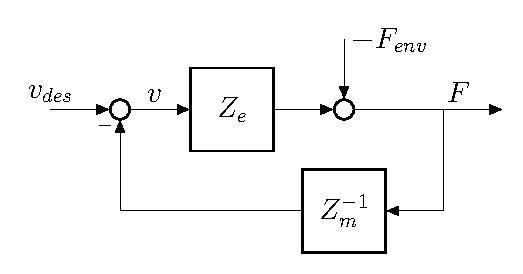
\includegraphics[scale=0.9]{position_control_feedback.pdf}
  \caption{Position control feedback. \label{fig:position_control_feedback}}
\end{figure}.
The commanded acceleration can be obtained from the velocity $v$ as
\[
a = \frac{\mathrm{d}}{\mathrm{d}t} \left(v_{des} - \frac{F}{Z_m}\right)
\]
In practice, the control $a$ can be obtained without use of differentiators
using only the measured force $F$, the end-effector position $x$ and velocity $\dot{x}$.
This is possible only if the manipulator impedance is expressed in a special form
\[
Z_m = Ms + \tilde{Z}_{m}
\]
where $M$ is a tuning parameter.
\par
Finally the position control law evaluates to
\begin{equation}
  \label{eq:position_law}
  a = \dot{v}_{des} + (v_{des} - v)\frac{\tilde{Z}_m}{M} - \frac{F}{M}
\end{equation}

\subsubsection{Force control}
The transfer function for the force-controlled circuit given in Equation (\ref{eq:force_control_circuit})
can also be realized as a force feedback scheme.
Figure \ref{fig:force_control_feedback} shows a block diagram of the force-control implementation.
\begin{figure}[h]
  \centering
  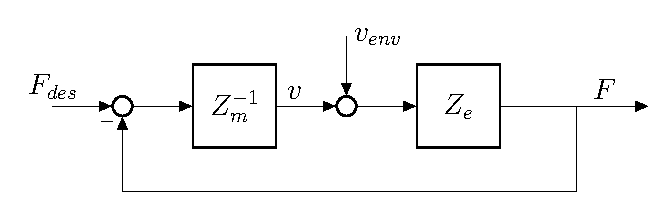
\includegraphics[scale=0.9]{force_control_feedback.pdf}
  \caption{Force control feedback. \label{fig:force_control_feedback}}
\end{figure}
Again the commanded acceleration can be obtained from the velocity $v$ as
\[
a = \frac{\mathrm{d}}{\mathrm{d}t} \left(\frac{F - F_{des}}{Z_m} \right)
\]
As done before for the position-controlled DoF $a$ can be obtained without differentiators if
the manipulator impedance assume the form
\[
Z_m = Ms + \tilde{Z}_{m}
\]
The force control law can then be written as
\begin{equation}
  \label{eq:force_law}
  a = \frac{1}{M} (F - F_{des}) - \frac{1}{M}( \tilde{Z}_m v)
\end{equation}

\subsection{Design of the control law}
In order to fulfill the control objectives described in \ref{sec:desired_dyn}
the manipulator impedances were chosen as follow.
\par
For the position and attitude-controlled DoFs they are
\[
\begin{split}
  &Z_{m,p} = M_p s + \tilde{Z}_{m,p} = M_p s + B_p + \frac{K_p}{s}\\
  &Z_{m,a} = M_a s + \tilde{Z}_{m,a} = M_a s + B_a + \frac{K_a}{s}
\end{split}
\]
which result in the following acceleration commands
\[
\begin{split}
  &a_{p} = a_{des,p} + \frac{B_p}{M_p} (v_{des,p} - v_p) + \frac{K_p}{M_p} (x_{des,p} - x_p) - \frac{F_p}{M_p}\\
  &a_a = a_{des,a} + \frac{B_a}{M_a} (v_{des,a} - v_a) + \frac{K_a}{M_a} (x_{des,a} - x_a) - \frac{F_a}{M_a}
\end{split}
\]
For the force-controlled DoF the impdance is given by
\[
Z_{m,f} = M_f s + \tilde{Z}_{m,f} = M_f s + B_f
\]
which results in the control law
\[  
a_{f} = M_f^{-1}((f_{des} - f) - B_f v_z)
\]
In principle a position control law and a force control law could be assigned for each DoF. Since this
behavior is not possible physically a selection matrix $S$ is used to separate the force-controlled and position-controlled reciprocal subspaces
\[
\vec{a} = S 
\begin{bmatrix}
  \vec{a}_p \\
  \vec{a}_a
\end{bmatrix} + (I - S) \vec{a}_f
\]
where the vector $\vec{a}_p$ and $\vec{a}_a$ are the position and attitude control laws
\[
\begin{split}
  &\vec{a}_p = 
  \begin{bmatrix}
    a_{p,x} & a_{p,y} & a_{p,z}
  \end{bmatrix}^T\\
  &\vec{a}_a = 
  \begin{bmatrix}
    a_{a, \psi} & a_{a, \theta} & a_{a, \phi}
  \end{bmatrix}^T
\end{split}
\]
the vector $\vec{a}_f$ is the force/torque control law
\[
\vec{a}_f = 
\begin{bmatrix}
  a_{f,x} & a_{f,y} & a_{f,z} & a_{f, \psi} & a_{f, \theta} & a_{f, \phi}
\end{bmatrix}^T
\]
and $S$ is the selection matrix that for the set-up described in section \ref{sec:task_description} assumes the form
\[
S =
\begin {bmatrix}
  1 & 0 & 0 & 0 & 0 & 0\\
  0 & 1 & 0 & 0 & 0 & 0\\
  0 & 0 & 0 & 0 & 0 & 0\\
  0 & 0 & 0 & 1 & 0 & 0\\
  0 & 0 & 0 & 0 & 1 & 0\\
  0 & 0 & 0 & 0 & 0 & 1\\
\end {bmatrix}
\]
The resulting control laws is
\begin{equation}\label{eq:final_a_cmd}
\begin{cases}
\prescript{ws}{}{a}_1 = a_x = \ddot{r}_{x,des} + B_x (\dot{r}_{x,des} - \dot{r}_x) + K_x (r_{x,des} - r_x) - F_x \\
\prescript{ws}{}{a}_2 = a_y = \ddot{r}_{y,des} + B_y (\dot{r}_{y,des} - \dot{r}_y) + K_y (r_{y,des} - r_y) - F_y \\
\prescript{ws}{}{a}_3 = a_z = - B_f \dot{r}_z + K_f(F_{z,des} - F_z) \\
\prescript{ws}{}{a}_4 = a_{\psi} = \ddot{\psi}_{des} + B_{\psi} (\dot{\psi}_{des} - \dot{\psi}) + K_{\psi} (\psi_{des} - \psi) \\
\prescript{ws}{}{a}_5 = a_{\theta} = \ddot{\theta}_{des} + B_{\theta} (\dot{\theta}_{des} - \dot{\theta}) + K_{\theta} (\theta_{des} - \theta) \\
\prescript{ws}{}{a}_6 = a_{\phi} = \ddot{\phi}_{des} + B_{\phi} (\dot{\phi}_{des} - \dot{\phi}) + K_{\phi} (\phi_{des} - \phi)
\end{cases}
\end{equation}
where the ratios of the form $\frac{K}{M}$ or $\frac{B}{M}$ are substituted with $K$ and $B$ respectively.
\par
The desired trajctories for the position and attitude-controlled DoFs were chosen as  $5^\text{th}$ order polynomials of the form
\[
s(t) = a_5 t^5 + a_4 t^4 + a_3 t^3 + a_2 t^2 +a_1 t + a_0
\]
with boundary conditions
\[
\begin{split}
  &s(0) = s_0 \quad \dot{s}(0) = 0 \quad \ddot{s}(0) = 0\\
  &s(t_f) = s_f \quad \dot{s}(t_f) = 0 \quad \ddot{s}(t_f) = 0
\end{split}
\]
while the reference force trajectory was chosen as a $3^\text{th}$ order polynomial
\[
s(t) = a_3 t^3 + a_2 t^2 +a_1 t + a_0
\] 
with boundary conditions
\[
\begin{split}
  &s(0) = s_0 \quad \dot{s}(0) = 0\\
  &s(t_f) = s_f \quad \dot{s}(t_f) = 0
\end{split}
\]
\newpage
